\chapter{CPU allocation and scheduling for containerized processes}
\lhead{Chapter 3. \emph{CPU allocation and scheduling for containerized processes}}
\label{cpuallocation}

\section{Goal of the experiment}

This experiment has been defined to study of the ability to isolate containers
CPU usage using Linux control groups Linux containers are sharing the same
operating system, they are not fully isolated as we can see with complete
virtual machines. To achieve this isolation, the control groups (cgroup) of the
linux kernel are used to apply limits on the resource access right of each
container.

This experiment aims at studying how these cgroups are working and how do they
actually share and isolate the CPU resources among the different containers.

\section{Metrics}

\subsection{Inputs}

The number of CPUs that an application consumes has to be clearly defined. In
each container, an application developed to consume a given number of CPU
cores will be launched. The source code of the application can be found at
\url{https://github.com/Soulou/msc-thesis-cpu-burn}.

\vspace{1em}
\lstset{language=bash}

\begin{lstlisting}
# Parameter n: Number of core to consume
./msc-thesis-cpu-burn -nb-cpus=<n>
\end{lstlisting}

The second input corresponds to the number of shares a container can access
on the CPUs of the running computer. This number is arbitrary as the shares
are relative to each other. 

\begin{quote}
If a container does not have any cpu share number specified, the default value
is: $1024$
\end{quote}

It is expected that if there are two containers, one with $1024$ cpu shares and
the other with $2048$ CPU shares, the second container will have access to
$2048/1024 = 200\%$ of the resources, for a single CPU: $33\%$ and $66\%$.

\subsection{Output}

As the input concerns the maximal CPU usage, the output the experiment is going
to get, each second, the actual consumption of each running container.

\section{Setup}

\subsection{Hosts}

To test the capacity of the isolation by cpu shares, two different environments
will be used. As the result are expected to be relative to the hardware their
should not be any major differences between both, but as a sanity test, it is
important execute it on two différents contexts

The first one my personal laptop, here are its characteristics:

\begin{itemize}
	\item{CPU: Intel\textregistered \hspace{1pt} Core\texttrademark
	\hspace{1pt} i7-3537U CPU @ 2.00GHz (2 cores with hyperthreading)}
	\item{Memory: 8 GB RAM DDR3}
	\item{Disk: 256GB Solid State Drive}
\end{itemize}

Then we'll study the results of the same experiment on a 4 cores virtual
machine based on an OpenStack cluster:

\begin{itemize}
	\item{CPU: 4 KVM vCPUs}
	\item{Memory: 8 GB RAM}
	\item{Disk: Virtual HDD 80GB}
\end{itemize}

\subsection{Deployment}

In order to simplify the reproduction of these experiments, the different
applications have been packaged into container images. They can be found on the
docker public repository:

\begin{itemize}
	\item{\texttt{soulou/msc-thesis-cpu-burn}}
	\item{\texttt{soulou/msc-thesis-docker-cpu-monitor}}
\end{itemize}

In order to deploy them, simply install Docker on your host
(\url{http://docs.docker.com/installation/}), then use the \texttt{docker pull}
to get the container images locally.

\vspace{1em}

\begin{lstlisting}
docker run -d soulou/msc-thesis-cpu-burn -nb-cpus=<n>
...
# Run more instances according to what your want to test
...
docker run -i -t \
  -v /var/run/docker.sock:/var/run/docker.sock \
  -v /sys/fs/cgroup/cpuacct/docker:/cgroup \
  soulou/msc-thesis-docker-cpu-monitor -cgroup-path=/cgroup
\end{lstlisting}

The cpu monitoring service will display in columns the cpu consumption
of each container running on the host (including itself), the data are
displayed to be quickly usable by a third-party data analysis tool like
\textbf{R} or to draw graph with \textbf{Gnuplot}

\section{Expected results}

Four different experiments have been done:

\begin{itemize}
\item{4 Processes with equal CPU shares : \newline The tested hosts
	have a total of 4 cores, normally 4 processes using 1 core each should
	be able to share it equally, and each of the process should be able to
	get 100\%
}
\item{4 Processes with different CPU shares 128-256-512-1024 : \newline
	For the same reason as the previous experiment, the
	shares should not change the results. Even if some processes have less
	priority over the CPU, as there is enough cores for all the processes,
	they should all be able to run their process at its maximum potential.
}
\item{6 processes with equal CPU shares : \newline This case is
	different, as there is a higher number of processes compared to the
	amount of available computation units. With an equal amount of CPU
	shares for each process, it is expected that each process will get 66\%
	in average of CPU time.  The results can't be stable as the mount of
	cores is not a divisor of the number of applications. In other words,
	there is no way the operating system can allocate an equal share of
	core per process, as the context of a process is linked to one core. An
	application can't be 33\% on one core, and 33\% on the other one at the
	same time.
}
\item{6 processes with different CPU shares 32-64-128-256-512-1024 : \newline
	According to the rule defined previously, a process with 64 shares
	should have twice more CPU time than a process with 32 shares but twice
	less than a 128-shares process.
}
\end{itemize}

\section{Results}

All the following graphs represent the percentage of CPU time per process
in function of the time in seconds.

\section{On the laptop}

\begin{figure}[h!]
\begin{center}
	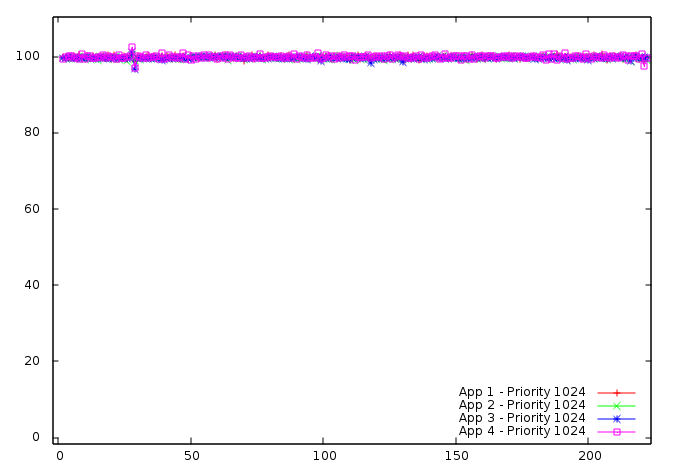
\includegraphics[width=0.45\textwidth]{./Images/CpuMonitor/laptop/4_equalshares.png}
	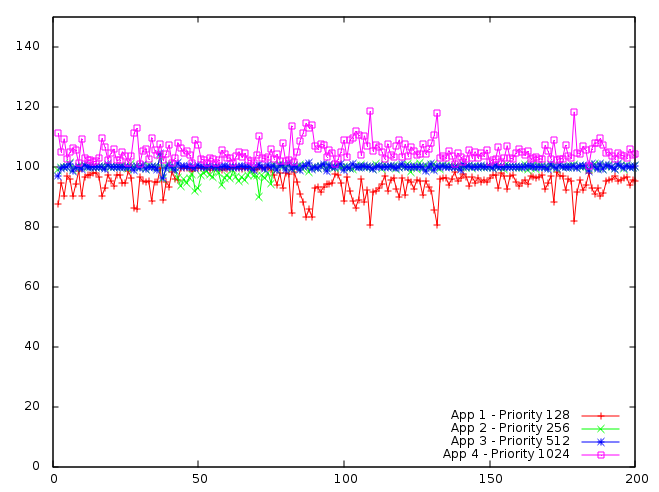
\includegraphics[width=0.45\textwidth]{./Images/CpuMonitor/laptop/4_differentshares.png}
	\caption{4 Processes with equal[1] and different[2] CPU shares}
\end{center}
\end{figure}

Using 4 processes, the expectations are reached, even if there are some small
differences between the execution with equal shares and the one without, it is
clear that each service can use one complete core whatever are its CPU shares.

\begin{figure}[h!]
\begin{center}
	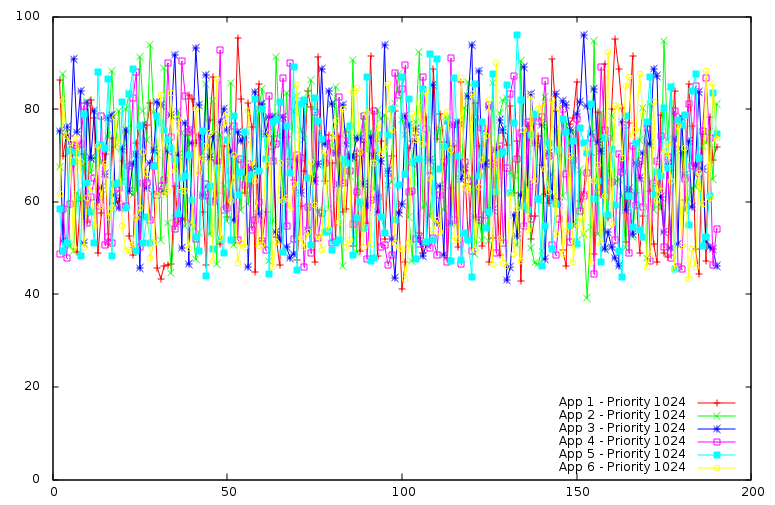
\includegraphics[width=0.45\textwidth]{./Images/CpuMonitor/laptop/6_equalshares.png}
	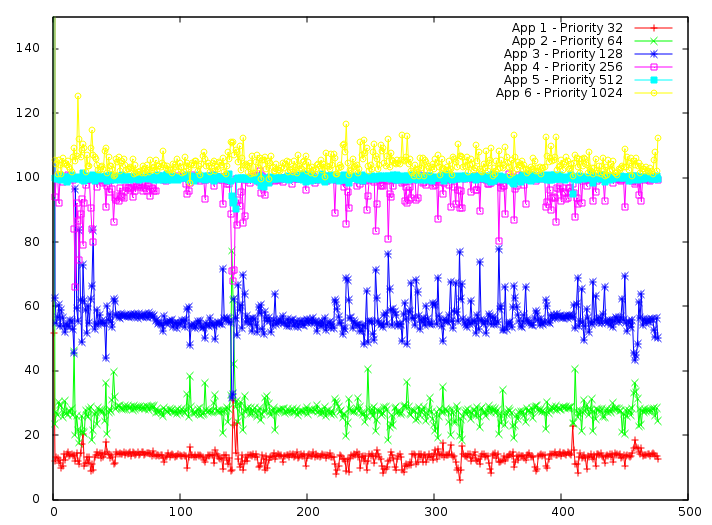
\includegraphics[width=0.45\textwidth]{./Images/CpuMonitor/laptop/6_differentshares.png}
	\caption{6 Processes with equal[1] and different[2] CPU shares}
\end{center}
\end{figure}

When 6 processes are executing on the host the observed behavior is different.
When shares are equal, the cpu consumption of each process is completely
unstable.  As explain in the expectation for this experiment, theoretically
each process should have 66\%, but as it's not possible because a process is
only attached to one core at a precise time, the operating system is moving the
processes during all the calculations. This is why the curves are so changing.
But overall, if we measure the average and median of the CPU consumption of
each application, the result is 66\%, so the expectation is reached.

In the case where 6 processes are running with different CPU shares, the
results are linked to what has been planned, but not only. The process with the
minimum amount of shares (32) is using $\approx15\%$ of CPU, then the one with
64 shares has $\approx30\%$ of CPU consumption, and then, the third one has
$\approx60\%$ of processor usage. These values are effectively each time twice
higher as the previous one. However this rule is not respected afterwards. Three
of the process are able to use one full core event if their shares are respectively
really different (256, 512, 1024)

\section{On the virtual machine}

As previously said, the results of this experiment in another environment should
not be fundamentally different. As the results are relative percentages, the
same figures should be found.

\begin{figure}[h!]
\begin{center}
	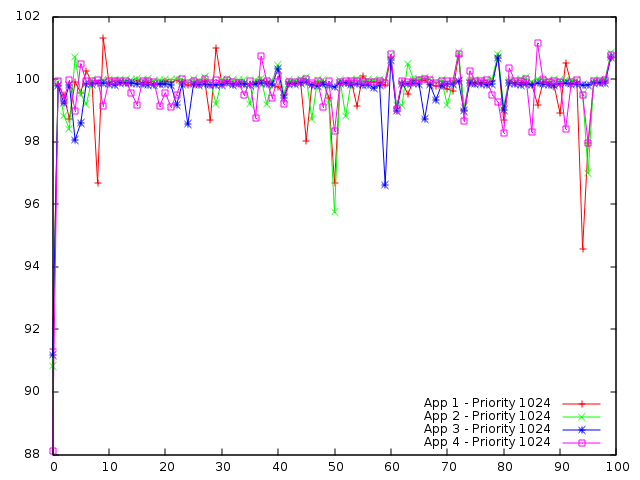
\includegraphics[width=0.45\textwidth]{./Images/CpuMonitor/vm/4_equalshares.png}
	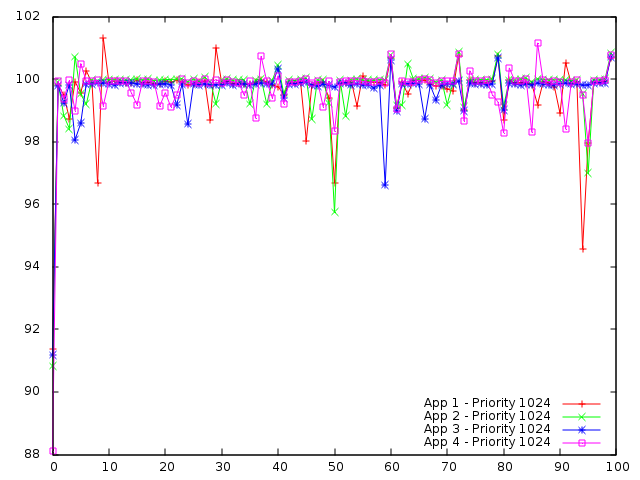
\includegraphics[width=0.45\textwidth]{./Images/CpuMonitor/vm/4_differentshares.png}
	\caption{4 Processes with equal[1] and different[2] CPU shares}
\end{center}
\end{figure}

When 4 processes are running, the results are not fundamentally different with
the previous ones. There are some instability which may be linked to the virtual
machine environment, but concretely, each process got 100\% of a core.

\begin{figure}[h!]
\begin{center}
	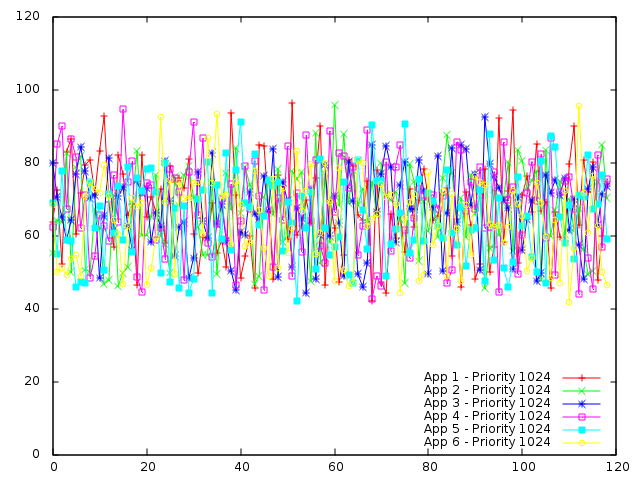
\includegraphics[width=0.45\textwidth]{./Images/CpuMonitor/vm/6_equalshares.png}
	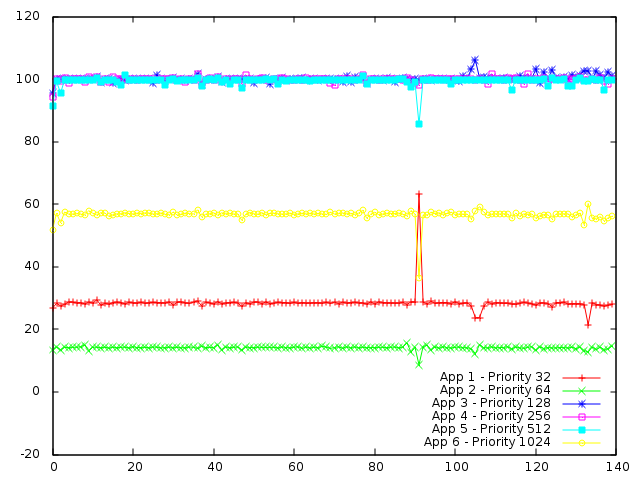
\includegraphics[width=0.45\textwidth]{./Images/CpuMonitor/vm/6_differentshares.png}
	\caption{6 Processes with equal[1] and different[2] CPU shares}
\end{center}
\end{figure}

Once more, the results are what we could expect. It is interesting that the
consumption of 6 processes looks much more constant in this environment. It
may be interesting to investigate that in order to know if it's because there
are less applications running on the server than the laptop or if the vCPUs used
by the virtual machine are rounding of the real CPU consumption on the physical
host provided by the hypervisor. It doesn't change fundamentally the results,
but there is a difference.

\section{Additional analysis}

We have seen that with 6 processes on 4 cores, 3 of them are able to get a full
CPU, in this case the processes are limiting the experiment. That is why, the 
operation has been repeated with the following parameters.

\begin{lstlisting}
docker run -d -c <shares> soulou/msc-thesis-cpu-burn -nb-cpus 2
\end{lstlisting}

In this case, each container will try to get 2 cores, so 200\% of CPU.

\begin{figure}[h1]
\begin{center}
	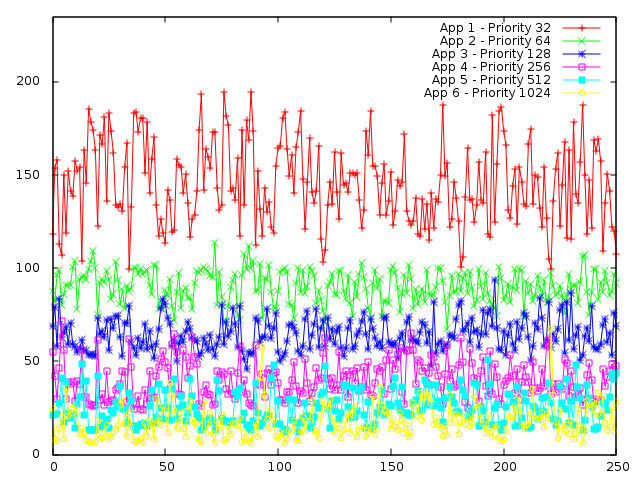
\includegraphics[width=0.6\textwidth]{./Images/CpuMonitor/vm/6_differentshares_2cores.png}
	\caption{6 Processes using 2 cores with different CPU shares}
\end{center}
\end{figure}

\vspace{2em}

\begin{center}
\begin{tabular}{l | c | c | c | c | c | c}
		& App6 & App5 & App4 & App3 & App2 & App1 \\
	Median  & 144.0 & 90.11 & 63.29 & 38.58 & 23.59 & 16.04 \\
	Mean    & 145.6 & 90.22 & 64.48 & 40.20 & 25.07 & 17.52
\end{tabular}
\captionof{table}{Median and mean of the different application CPU usage in \%}
\end{center}

Compared to the previous experiment, we can first observe that the limit is not
the process anymore, none of the applications have reached their maximal
potential 200\%. However, the observed relation between two tasks has been
lost. The more shares it owns, the more CPU usage a process has, accordingly to
the shares. The operating system is respecting the shares, in a best effort.
The priority of one process over another can not be precisely defined.

\section{Conclusion on the experiment}

The main goal of this experiment was to show that it is possible to give different
priority levels to different applications running on a given host. This is something
really important because in the scope of multiuser infrastructure, resources
should be manageable. The \textbf{cgroups} already allow to set hard limit on memory
consumption, but the CPU limits are different. The \textbf{cgroup} cpuset has not
been mentioned in this experiment, it is another solution for CPU resource
management but it is not integrated in \textbf{docker}. The \textbf{docker} developers
are currently working on the addition of more resource control features but as the project
is still quite recent, they are still not implemented.

The obtained results are in line with the expectations, as long as there is less processes
than cores, the shares have no effect, but when the relation changes and the number of
processes is increasing, the shares can have an important impact on how an application
will be able to use the available cores. From a Quality of Service perspective, it allows
to regulate the processes on a server base, to decrease the "Bad neighbour" effect, when
one or different processes are slowing down all the other processes of a host.
